%%%%%%%%%%%%%%%%%%%%%%%%%%%%%%%%%
%% Template released under AGPLv3 by Andrew Rechnitzer (c) 2019
%% This template uses latex exam class.
%%%%%%%%%%%%%%%%%%%%%%%%%%%%%%%%%

\documentclass[12pt]{exam}

%%%%%%%%%%%%%%%%%%%%%%%%%%%%%%%%%%%%%%%%%%%%%%%%%%%%
%% This template is for letter-paper, not a4 paper.
%% The margins have been set so as to work nicely
%% with the QR-codes etc needed by Plom.
%%
%% It has also been designed to use the latex exam class
%% which auto-computes totals etc and also makes it easy
%% for the instructor to include solutions in their .tex
%% We recommend that you use this.


\boxedpoints
\marksnotpoints
\addpoints
\extrawidth{-20mm}


%%%%%%%%%%%%%%%%%%%%%%%%%%%%%%%
% If we want to print out the answers/solns then we should
% also NOT print those extra spaces and blankpages.
% To help us do this we define a boolean flag
% By default we have it set to true, telling latex to put
% in the extra spacing etc.
\newboolean{space} \setboolean{space}{true}

%% Now, to print answers/soln and remove the extra spacing
%% just comment out the line below
%% vvvvvvv
%% vvvvv
%% vvv
%% v

% \printanswers  \setboolean{space}{false}

%% ^
%% ^^^
%% ^^^^^
%% ^^^^^^^
%% Try running this with and without the line above

%%%%%%%%%%%%%%%%%%%%%%%%%%%%%%%%%%%%%%%%%%%%%%%%%%%%
% Here are some handy commands for adding spacing / blank pages / answerboxes
% when printing with or without solns.

% Use this to put a vfill between things when printing
% without answers/solutions. No space when printing with answers/solns
\newcommand{\blank}{
  \ifthenelse{\boolean{space}}{\vfill}{}
}

% Use this to put a blankpage when printing
% without answers/solutions. No page when printing with answers/solns
\newcommand{\blankpage}{
\ifthenelse{\boolean{space}}{
\pagebreak
\emph{This page has been left blank for your workings and solutions.}
\pagebreak
}{} }

% Use this to make a nice answerbox which will display the correct answer
% when solutions are printed and is otherwise blank for the students
% to write their stuff.
\newcommand{\answerbox}[1]{
\begin{flushright}
\fbox{\parbox[l]{60mm}{Answer:
\ifthenelse{\boolean{space}}{\vspace{10mm}}{#1}{}} }
\end{flushright}
}
% A slightly larger answerbox
\newcommand{\Answerbox}[1]{
\begin{flushright}
\fbox{\parbox[l]{80mm}{Answer:
\ifbool{space}{\vspace{10mm}}{#1}{}} }
\end{flushright}
}



%%%%%%%%%%%%%%%%%%%%%%%%%%%%%%%%%
%% Load packages and things here
\usepackage{amsmath,amsthm,amsfonts,amssymb}
\usepackage{enumerate}
\usepackage{graphicx}

%%%%%%%%%%%%%%%%%%%%%%%%%%%%%%%%%
% Make the header blank, but put page info in the footer.
\chead{}
\cfoot{Page \thepage\ of \numpages}


%%%%%%%%%%%%%%%%%%%%%%%%%%%%%%%%%
%% Your macros should go here


%%%%%%%%%%%%%%%%%%%%%%%%%%%%%%%%%
%% Time to start the actual test

\begin{document}

\section*{Mathematics ABC --- Midterm --- 45 minutes}
\subsection*{October 43th 2318}
\begin{itemize}
  \item The test consists of \numpages\ pages and \numquestions\ questions worth a total of \numpoints\ marks.
  \item This is a closed-book examination. \textbf{None of the following are allowed}: documents, cheat sheets or electronic devices of any kind (including calculators, \underline{cell phones}, etc.)
  \item No work on this page will be marked.
  \item Fill in the information below before turning to the questions.
\end{itemize}

\begin{center}
  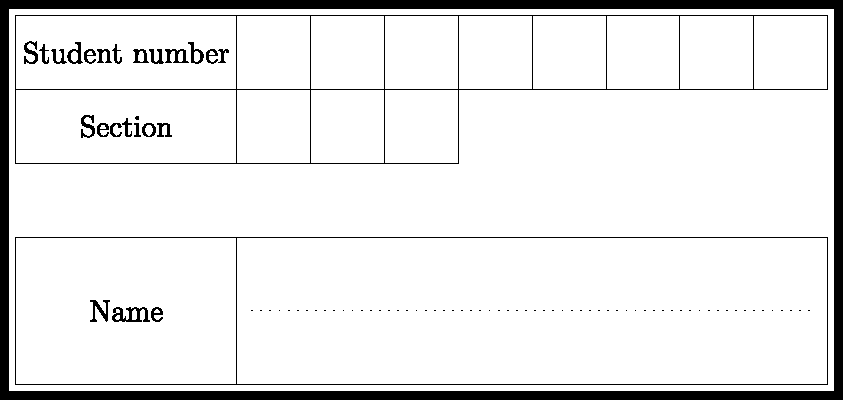
\includegraphics{idBox2}
\end{center}


\vfill
\newpage

\begin{questions}
\question[5] Please place your answers in the boxes provided
\begin{parts}
  \part Answer something simple
  \answerbox{ABC}
  \begin{solution}
    Some working will go here.
  \end{solution}
  \blank
  % Use \blank to space out the question parts nicely.

  \part Another little thing here.
  \answerbox{\(\sin(x)\)}
  \begin{solution}
    Putting in your solutions ahead of time really helps calibrate your test.
  \end{solution}
  \blank

  \part A third thing
  \answerbox{\(\int \sin(x) dx\)}
  \begin{solution}
    Yet another solution goes here.
  \end{solution}
  \blank
\end{parts}
\newpage

%% Next question

\question[10] A long question goes here. In fact it is sufficiently long that we make sure you have a whole extra blank page for your work.
\begin{solution}
  A long solution here. Maybe it even contains a diagram?
\end{solution}

\blankpage

\end{questions}
\end{document}
